\documentclass[11pt,a4paper]{scrartcl}

% ============================================
% Pakete
% ============================================
\usepackage[utf8]{inputenc}
\usepackage[T1]{fontenc}
\usepackage[ngerman]{babel}
\usepackage{amsmath,amssymb}
\usepackage{siunitx}
\sisetup{locale=DE, per-mode=fraction}
\usepackage{graphicx}
\usepackage{booktabs}
\usepackage{array}
\usepackage{tcolorbox}
\tcbuselibrary{skins, breakable}
\usepackage{fontawesome5}
\usepackage{tikz}
\usetikzlibrary{shapes.geometric, arrows.meta, positioning}
\usepackage{scrlayer-scrpage}
\usepackage{geometry}
\geometry{left=2.5cm, right=2.5cm, top=3cm, bottom=2.5cm, headheight=1.5cm}

% ============================================
% Kopf- und Fußzeile (KOMA-Script)
% ============================================
\clearpairofpagestyles
\ihead{
\includegraphics[height=1cm]{logo.jpeg}}
\chead{\textbf{Physik-LK 11NP}}
\ohead{\textbf{\today}}
\cfoot{\pagemark}
\KOMAoptions{headsepline=0.4pt}

% ============================================
% tcolorbox-Definitionen
% ============================================
\newtcolorbox{formelbox}[1][]{
	colback=blue!5!white,
	colframe=blue!75!black,
	fonttitle=\bfseries,
	title={\faIcon{square-root-alt} Formel},
	#1
}

\newtcolorbox{aufgabe}[1][]{
	colback=orange!5!white,
	colframe=orange!75!black,
	fonttitle=\bfseries,
	title={\faIcon{pencil-alt} Aufgabe},
	#1
}

\newtcolorbox{sternaufgabe}[1][]{
	colback=red!5!white,
	colframe=red!75!black,
	fonttitle=\bfseries,
	title={\faIcon{star} Sternaufgabe},
	#1
}

\newtcolorbox{hilfebox}[1][]{
	colback=green!5!white,
	colframe=green!60!black,
	fonttitle=\bfseries,
	title={\faIcon{lightbulb} Hinweis},
	#1
}

\newtcolorbox{infobox}[1][]{
	colback=gray!5!white,
	colframe=gray!75!black,
	fonttitle=\bfseries,
	title={\faIcon{info-circle} Information},
	#1
}

\newtcolorbox{materialbox}[1][]{
	colback=purple!5!white,
	colframe=purple!75!black,
	fonttitle=\bfseries,
	title={\faIcon{tools} Materialien},
	#1
}

\setlength{\parindent}{0pt}
\setlength{\parskip}{0.5em}

% ============================================
% Dokumentbeginn
% ============================================
\begin{document}
	
	% ============================================
	% Titel
	% ============================================
	\begin{center}
		{\LARGE\bfseries Experiment 5: Wärmeenergie}\\[0.5cm]
		{\large Bestimmung der spezifischen Wärmekapazität von Wasser}
	\end{center}
	
	\vspace{0.5cm}
	
	% ============================================
	% Theoretischer Hintergrund
	% ============================================
	\section*{Theoretischer Hintergrund}
	
	Bei der Umwandlung einer Energieform in eine andere entsteht im Allgemeinen auch \textbf{Wärmeenergie}. Wandelt man z.\,B. in einer Glühlampe elektrische Energie in Lichtenergie um, so wird sie warm -- es entsteht Wärmeenergie. Fließt ein elektrischer Strom $I$ durch einen Draht, so wird dieser warm.
	
	Damit ein möglichst großer Teil der elektrischen Energie, die im Widerstandsdraht in Wärme umgewandelt wird, von dem untersuchten Körper aufgenommen wird, benutzt man zweckmäßigerweise eine Flüssigkeit, weil sie den Draht ganz umschließt.
	
	\begin{center}
		\begin{tikzpicture}[scale=1.0, every node/.style={font=\small}]
			% Linker Pfeil (Elektrische Energie) - Pfeil zeigt NACH rechts
			\fill[black] (0,0.5) -- (0,-0.5) -- (2,0) -- cycle;
			\node[above] at (1,0.7) {$U \cdot I \cdot t$};
			\node[below] at (1,-0.9) {Elektrische Energie};
			
			% Kasten (Energie-Umwandlung)
			\draw[thick] (2.2,-0.8) rectangle (5.8,0.8);
			\node[align=center] at (4,0) {\textbf{Energie-}\\\textbf{umwandlung}};
			
			% Rechter Pfeil (Wärmeenergie) - Pfeil zeigt NACH rechts
			\fill[black] (6,0.5) -- (6,-0.5) -- (8,0) -- cycle;
			\node[above] at (7,0.7) {$m \cdot c \cdot \Delta T$};
			\node[below] at (7,-0.9) {Wärmeenergie};
		\end{tikzpicture}
	\end{center}
	
	Die Temperaturerhöhung ist proportional zur zugeführten Energie $W$ und hängt neben der Masse $m$ auch von der Art des Materials ab. Dies wird durch die \textbf{spezifische Wärmekapazität} $c$ ausgedrückt:
	
	\begin{formelbox}[title={\faIcon{square-root-alt} Wärmeenergie}]
		\[W = c \cdot m \cdot \Delta T\]
		
		\textbf{Dabei gilt:}
		\begin{itemize}
			\item $W$ -- zugeführte Energie in J
			\item $c$ -- spezifische Wärmekapazität in $\si{\joule\per\gram\per\kelvin}$
			\item $m$ -- Masse in g
			\item $\Delta T$ -- Temperaturänderung in K (bzw. °C)
		\end{itemize}
	\end{formelbox}
	
	\begin{infobox}[title={\faIcon{info-circle} Spezifische Wärmekapazität von Wasser}]
		Für Wasser gilt:
		\[c_{\text{Wasser}} = \SI{4,19}{\joule\per\gram\per\kelvin} = \SI{4,19}{\kilo\joule\per\kilogram\per\kelvin}\]
		
		Das bedeutet: Um \SI{1}{\gram} Wasser um \SI{1}{\kelvin} zu erwärmen, benötigt man \SI{4,19}{\joule} Energie.
	\end{infobox}
\begin{hilfebox}[title={\faIcon{lightbulb} Umrechnung °C in K}]
	Der Zusammenhang zwischen Celsius und Kelvin lautet:
	\[T \text{ in K} = T \text{ in } ^\circ\text{C} + 273{,}15\]
	
	Eine Temperaturdifferenz in Grad Celsius entspricht jedoch zahlenmäßig der Temperaturdifferenz in Kelvin:
	\[\Delta T \text{ in } ^\circ\text{C} = \Delta T \text{ in K}\]
	Beispiel: Eine Erwärmung von \SI{20}{\celsius} auf \SI{35}{\celsius} ergibt $\Delta T = \SI{15}{\kelvin}$.
	
	\textbf{Absoluter Nullpunkt:} \SI{0}{\kelvin} $=$ \SI{-273,15}{\celsius} -- die tiefstmögliche Temperatur, bei der alle Teilchenbewegung zum Erliegen kommt.
\end{hilfebox}
	\begin{formelbox}[title={\faIcon{square-root-alt} Elektrische Energie}]
		Die zugeführte elektrische Energie berechnet sich aus:
		\[W_{\text{el}} = U \cdot I \cdot t\]
		
		\textbf{Dabei gilt:}
		\begin{itemize}
			\item $U$ -- Spannung in V
			\item $I$ -- Stromstärke in A
			\item $t$ -- Zeit in s
		\end{itemize}
	\end{formelbox}
	
	% ============================================
	% Versuchsaufbau
	% ============================================
	\section*{Versuchsaufbau}
	
	\begin{materialbox}
		\begin{minipage}{0.48\textwidth}
			\begin{itemize}
				\item Kalorimeter (Dewar-Gefäß)
				\item Heizwiderstand ($2 \times \SI{1}{\ohm}$)
				\item Spannungsquelle
			\end{itemize}
		\end{minipage}
		\begin{minipage}{0.48\textwidth}
			\begin{itemize}
				\item Amperemeter
				\item Voltmeter
				\item Thermometer / Zeitmesser
			\end{itemize}
		\end{minipage}
	\end{materialbox}
	
	\vspace{0.3cm}
	
	\begin{figure}[h]
		\centering
		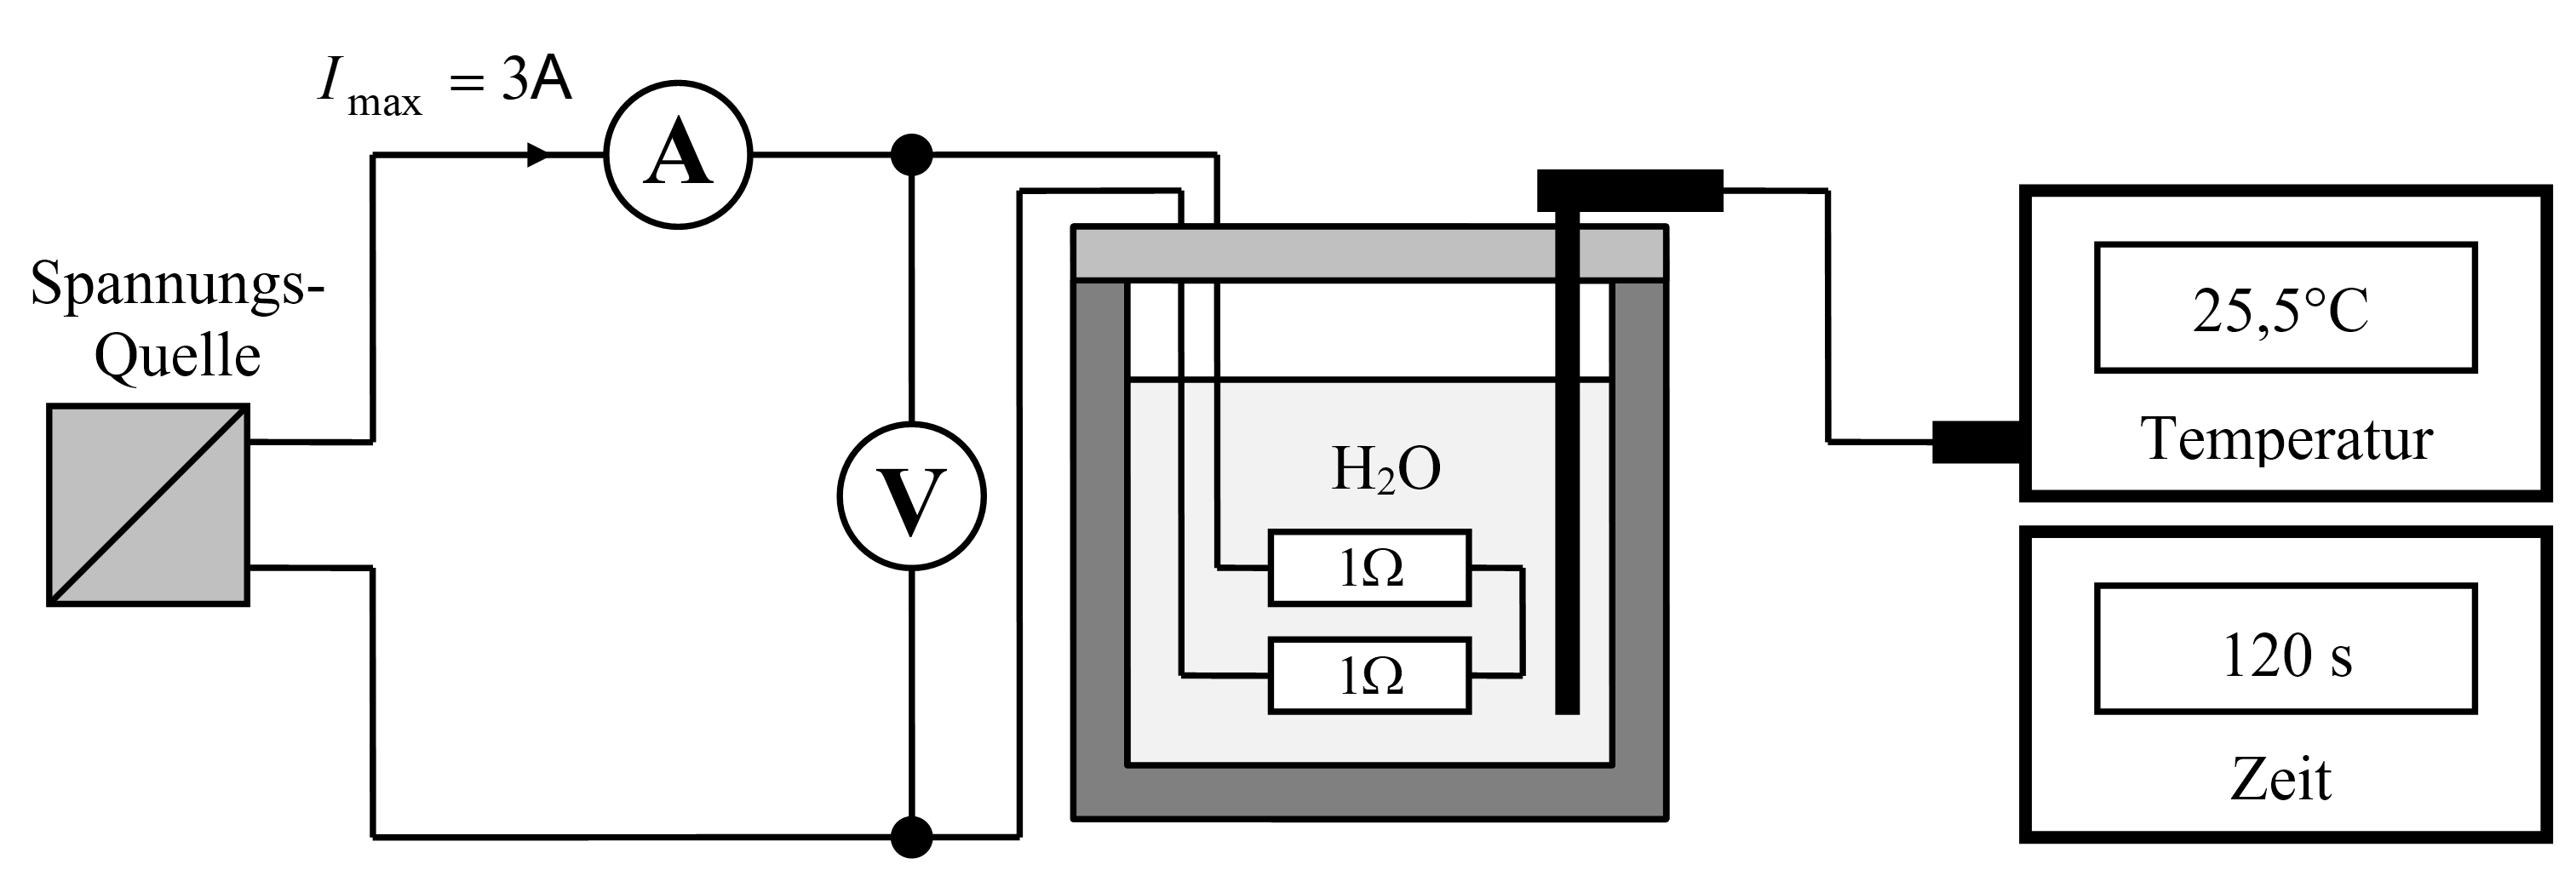
\includegraphics[width=0.85\textwidth]{dewar.png}
		\caption{Versuchsaufbau mit Kalorimeter, Heizwiderstand und Messgeräten}
		\label{fig:dewar}
	\end{figure}
	
	\begin{hilfebox}[title={\faIcon{lightbulb} Hinweise zum Aufbau}]
		\begin{itemize}
			\item Der maximale Strom beträgt $I_{\text{max}} = \SI{3}{\ampere}$ -- nicht überschreiten!
			\item Die Heizspirale muss \textbf{vollständig} unter Wasser sein.
			\item Das Wasser während der Messung gelegentlich umrühren.
			\item Das Dewar-Gefäß minimiert Wärmeverluste an die Umgebung.
		\end{itemize}
	\end{hilfebox}
	
	% ============================================
	% Versuchsprinzip
	% ============================================
	\section*{Versuchsprinzip}
	
	In diesem Experiment wird der Zusammenhang zwischen der zugeführten elektrischen Energie und der dadurch hervorgerufenen Temperaturänderung untersucht. Bauen Sie den Versuch gemäß Abbildung~\ref{fig:dewar} auf. Es werden zwei Versuchsreihen durchgeführt:
	
	\textbf{Versuchsteil 1:} Temperaturerhöhung bei konstanter Wassermasse\\
	\textbf{Versuchsteil 2:} Zeit für konstante Temperaturerhöhung bei verschiedenen Wassermassen
	
	% ============================================
	% Aufgabenstellungen
	% ============================================
	\section*{Aufgabenstellungen}
	
	\subsection*{Versuchsteil 1: Konstante Wassermasse}
	
	Das Kalorimeter wird mit \SI{200}{\gram} Leitungswasser gefüllt.
	
	\begin{aufgabe}[title={\faIcon{pencil-alt} Aufgabe 1.1: Messung}]
		Notieren Sie über insgesamt etwa \textbf{15 Minuten} die Temperatur und die verstrichene Zeit alle \textbf{zwei Minuten} in einer Tabelle mit Strom, Spannung, Zeit und Temperatur.
	\end{aufgabe}
	
	\begin{aufgabe}[title={\faIcon{pencil-alt} Aufgabe 1.2: Berechnung}]
		Berechnen Sie für jeden Messpunkt die bis dahin jeweils aufgewandte elektrische Energie:
		\[W_{\text{el}} = U \cdot I \cdot t\]
		Tragen Sie diese Energiewerte in die erweiterte Tabelle ein.
	\end{aufgabe}
	
	\begin{aufgabe}[title={\faIcon{pencil-alt} Aufgabe 1.3: Grafische Darstellung}]
		Stellen Sie die Energie $W$ als Funktion der Temperaturdifferenz $\Delta T$ grafisch dar und formulieren Sie den Zusammenhang zwischen Energiezufuhr und Temperaturerhöhung mathematisch.
	\end{aufgabe}
	
	\subsection*{Versuchsteil 2: Variable Wassermasse}
	
	Bei gleichem Versuchsaufbau wird untersucht, welche Zeit nötig ist, um verschiedene Wassermassen um die gleiche Temperaturdifferenz von \SI{10}{\celsius} zu erwärmen.
	
	\begin{aufgabe}[title={\faIcon{pencil-alt} Aufgabe 2.1: Messung}]
		Messen Sie die Zeiten (bei konstantem Strom und konstanter Spannung), die bei den Wassermassen \textbf{\SI{100}{\gram}, \SI{150}{\gram} und \SI{200}{\gram}} benötigt werden.
		
		\textbf{Achtung:} Die Heizspirale muss immer unterhalb der Wasseroberfläche bleiben!
	\end{aufgabe}
	
	\begin{aufgabe}[title={\faIcon{pencil-alt} Aufgabe 2.2: Berechnung und Darstellung}]
		Berechnen Sie für jede Messung die elektrische Energie und stellen Sie die Energie als Funktion der Masse dar ($W$-$m$-Diagramm).
	\end{aufgabe}
	
	\begin{aufgabe}[title={\faIcon{pencil-alt} Aufgabe 2.3: Interpretation}]
		Deuten Sie das Diagramm, indem Sie einen mathematischen Zusammenhang angeben.
	\end{aufgabe}
	
	\subsection*{Gesamtauswertung}
	
	\begin{aufgabe}[title={\faIcon{pencil-alt} Aufgabe 3.1: Gesamtzusammenhang}]
		Formulieren Sie mit Hilfe der beiden obigen Zusammenhänge den Gesamtzusammenhang zwischen Energie $W$, Wassermasse $m$ und Temperaturerhöhung $\Delta T$ als Proportionalgleichung.
	\end{aufgabe}
	
	\begin{aufgabe}[title={\faIcon{pencil-alt} Aufgabe 3.2: Bestimmung der Wärmekapazität}]
		Bestimmen Sie für alle Messungen aus beiden Versuchsreihen das Verhältnis:
		\[c = \frac{W}{m \cdot \Delta T}\]
	\end{aufgabe}
	
	\begin{sternaufgabe}[title={\faIcon{star} Aufgabe 3.3: Vergleich mit Literaturwert}]
		Berechnen Sie den Mittelwert von $c$ und vergleichen Sie Ihren Wert mit dem Literaturwert $c_{\text{Lit}} = \SI{4,19}{\joule\per\gram\per\kelvin}$. Geben Sie die prozentuale Abweichung an und nennen Sie Ursachen für diese Abweichung.
	\end{sternaufgabe}
	
	% ============================================
	% Protokollbogen
	% ============================================
	\newpage
	\section*{Protokollbogen -- Experiment 5}
	
	\begin{center}
		\begin{tcolorbox}[colback=white, colframe=black, width=\textwidth, boxrule=0.5pt]
			\begin{tabular}{@{}p{0.32\textwidth}p{0.32\textwidth}p{0.32\textwidth}@{}}
				\textbf{Name:} \hrulefill & \textbf{Klasse:} \hrulefill & \textbf{Datum:} \hrulefill \\[0.4cm]
				\textbf{Gruppenmitglieder:} & \multicolumn{2}{l}{\hrulefill} \\
			\end{tabular}
		\end{tcolorbox}
	\end{center}
	
	\subsection*{Versuchsteil 1: Konstante Wassermasse}
	
	\textbf{Wassermasse:} $m = \SI{200}{\gram}$ \hfill \textbf{Spannung:} $U = $ \rule{2cm}{0.4pt} V \hfill \textbf{Stromstärke:} $I = $ \rule{2cm}{0.4pt} A
	
	\vspace{0.3cm}
	
	\begin{center}
		\renewcommand{\arraystretch}{2.2}
		\begin{tabular}{|p{2.5cm}|p{1.3cm}|p{1.3cm}|p{1.3cm}|p{1.3cm}|p{1.3cm}|p{1.3cm}|p{1.3cm}|p{1.3cm}|}
			\hline
			\textbf{Zeit} $t$ in min & 0 & 2 & 4 & 6 & 8 & 10 & 12 & 14 \\
			\hline
			\textbf{Zeit} $t$ in s & 0 & 120 & 240 & 360 & 480 & 600 & 720 & 840 \\
			\hline
			\textbf{Temp.} $T$ in °C & & & & & & & & \\
			\hline
			$\Delta T$ in K & 0 & & & & & & & \\
			\hline
			$W_{\text{el}}$ in J & 0 & & & & & & & \\
			\hline
		\end{tabular}
	\end{center}
	
	\begin{infobox}[title={\faIcon{info-circle} Berechnung}]
		\textbf{Elektrische Energie:} \quad $W_{\text{el}} = U \cdot I \cdot t$
		
		\textbf{Temperaturdifferenz:} \quad $\Delta T = T - T_0$ \quad (mit $T_0$ = Anfangstemperatur)
	\end{infobox}
	
	\vspace{0.5cm}
	
	\subsection*{Versuchsteil 2: Variable Wassermasse}
	
	\textbf{Temperaturdifferenz:} $\Delta T = \SI{10}{\kelvin}$ \hfill \textbf{Spannung:} $U = $ \rule{2cm}{0.4pt} V \hfill \textbf{Stromstärke:} $I = $ \rule{2cm}{0.4pt} A
	
	\vspace{0.3cm}
	
	\begin{center}
		\renewcommand{\arraystretch}{2.5}
		\begin{tabular}{|p{4cm}|p{3cm}|p{3cm}|p{3cm}|}
			\hline
			\textbf{Messung Nr.} & \centering\textbf{1} & \centering\textbf{2} & \centering\arraybackslash\textbf{3} \\
			\hline
			Wassermasse $m$ in g & \centering 100 & \centering 150 & \centering\arraybackslash 200 \\
			\hline
			Zeit $t$ in s & & & \\
			\hline
			$W_{\text{el}} = U \cdot I \cdot t$ in J & & & \\
			\hline
		\end{tabular}
	\end{center}
	
	% ============================================
	% Protokollbogen Seite 2
	% ============================================
	\newpage
	
	\subsection*{Diagramm 1: $W$-$\Delta T$-Diagramm (Versuchsteil 1)}

	\begin{hilfebox}[title={\faIcon{lightbulb} Neu: Skalierung selbst wählen}]
		Ab diesem Versuch legen Sie die Achsenskalierung selbst fest:
		\begin{itemize}
			\item Größten Messwert bestimmen -- er muss noch auf das Gitter passen.
			\item Runde Schrittweite pro Kästchen wählen (1, 2, 5, 10, \dots).
			\item Zahlen an die dicken Gitterlinien schreiben -- Einheit nicht vergessen!
		\end{itemize}
	\end{hilfebox}

	
	\begin{center}
		\begin{tikzpicture}[scale=0.9]
			% Koordinatensystem
			\draw[->] (0,0) -- (12,0) node[right] {$\Delta T$ in K};
			\draw[->] (0,0) -- (0,9) node[above] {$W$ in J};
			
			% Gitternetz
			\draw[gray!30, very thin] (0,0) grid[step=0.5] (11.5,8.5);
			\draw[gray!50, thin] (0,0) grid[step=1] (11.5,8.5);
			
			% Achsenbeschriftung x
			
			% Achsenbeschriftung y
		\end{tikzpicture}
	\end{center}
	
	\subsection*{Diagramm 2: $W$-$m$-Diagramm (Versuchsteil 2)}
	
	\begin{center}
		\begin{tikzpicture}[scale=0.9]
			% Koordinatensystem
			\draw[->] (0,0) -- (12,0) node[right] {$m$ in g};
			\draw[->] (0,0) -- (0,9) node[above] {$W$ in J};
			
			% Gitternetz
			\draw[gray!30, very thin] (0,0) grid[step=0.5] (11.5,8.5);
			\draw[gray!50, thin] (0,0) grid[step=1] (11.5,8.5);
			
			% Achsenbeschriftung x
			
			% Achsenbeschriftung y
		\end{tikzpicture}
	\end{center}
	
	% ============================================
	% Protokollbogen Seite 3
	% ============================================
	\newpage
	
	\subsection*{Gesamtauswertung: Bestimmung der spezifischen Wärmekapazität}
	
	\begin{center}
		\renewcommand{\arraystretch}{2.5}
		\begin{tabular}{|p{3cm}|p{2cm}|p{2cm}|p{2cm}|p{2.5cm}|}
			\hline
			\textbf{Messung} & $W$ in J & $m$ in g & $\Delta T$ in K & $c = \frac{W}{m \cdot \Delta T}$ in $\frac{\text{J}}{\text{g}\cdot\text{K}}$ \\
			\hline
			VT1: $t = \SI{2}{min}$ & & 200 & & \\
			\hline
			VT1: $t = \SI{4}{min}$ & & 200 & & \\
			\hline
			VT1: $t = \SI{6}{min}$ & & 200 & & \\
			\hline
			VT1: $t = \SI{8}{min}$ & & 200 & & \\
			\hline
			VT1: $t = \SI{10}{min}$ & & 200 & & \\
			\hline
			VT2: $m = \SI{100}{g}$ & & 100 & 10 & \\
			\hline
			VT2: $m = \SI{150}{g}$ & & 150 & 10 & \\
			\hline
			VT2: $m = \SI{200}{g}$ & & 200 & 10 & \\
			\hline
		\end{tabular}
	\end{center}
	
	\vspace{0.5cm}
	
	\begin{tcolorbox}[colback=yellow!10!white, colframe=yellow!50!black, width=\textwidth]
		\centering
		\textbf{Ergebnis: Spezifische Wärmekapazität von Wasser}\\[0.3cm]
		{\Large $\bar{c} = \rule{3cm}{0.4pt}\;\si{\joule\per\gram\per\kelvin}$}
	\end{tcolorbox}
	
	\vspace{0.3cm}
	
	\textbf{Literaturwert:} $c_{\text{Lit}} = \SI{4,19}{\joule\per\gram\per\kelvin}$ \hfill \textbf{Relative Abweichung:} \rule{3cm}{0.4pt} \%
	
	\vspace{0.5cm}
	
	\subsection*{Zusammenhänge und Fehlerquellen}
	
	\textbf{Zusammenhang aus Versuchsteil 1:} $W \sim$ \rule{3cm}{0.4pt}
	
	\vspace{0.5cm}
	
	\textbf{Zusammenhang aus Versuchsteil 2:} $W \sim$ \rule{3cm}{0.4pt}
	
	\vspace{0.5cm}
	
	\textbf{Gesamtzusammenhang:}
	
	\vspace{1.5cm}
	
	\textbf{Fehlerquellen:}
	
	\vspace{4cm}
	

	% ============================================
	% Abgabevermerk (Rev. 1)
	% ============================================
	\vspace{0.4cm}
	\begin{tcolorbox}[colback=yellow!8, colframe=black, boxrule=0.6pt, title={\faIcon{check-circle}\enspace Abgabevermerk -- wird vor Ort ausgefüllt}, fonttitle=\bfseries]
		Abgegeben am \rule{2.8cm}{0.4pt} \enspace um \rule{2cm}{0.4pt} Uhr \hfill Sichtvermerk Lehrkraft: \rule{3.5cm}{0.4pt}

		\vspace{0.15cm}
		{\small\textit{Dieser Protokollbogen verbleibt in Ihrer \textbf{Praktikumsmappe}. Die vollständige Mappe wird am Ende des Schuljahres vorgelegt.} \hfill \scriptsize Rev.\,1}
	\end{tcolorbox}

\end{document}